%% ------------------------------------------------------------------------- %%
\chapter{Contexto Teórico}
\label{cap:conceitos}

Este capítulo apresenta, um a um, os conceitos mais elementares, 
e tenta harmonizar a terminologia empregada no decorrer do texto.


%% ------------------------------------------------------------------------- %%
\section{\Gls{tectonic}}
\index{\gls{tectonic}}
\label{sec:02_tectonica}

A \gls{tectonic} é um \glsdesc*{tectonic}.

Uma das principais evidências das transformações geológicas do planeta 
são os \glspl{equake}. A figura \ref{f:global_epicenters} \citep{img_world_epicenters}
é um mapa global com a ocorrência geográfica dos tremores. Nele é possivel notar que 
os sismos não são distribuídos uniformemente pelo globo.

\begin{figure}[H]
   \centering
   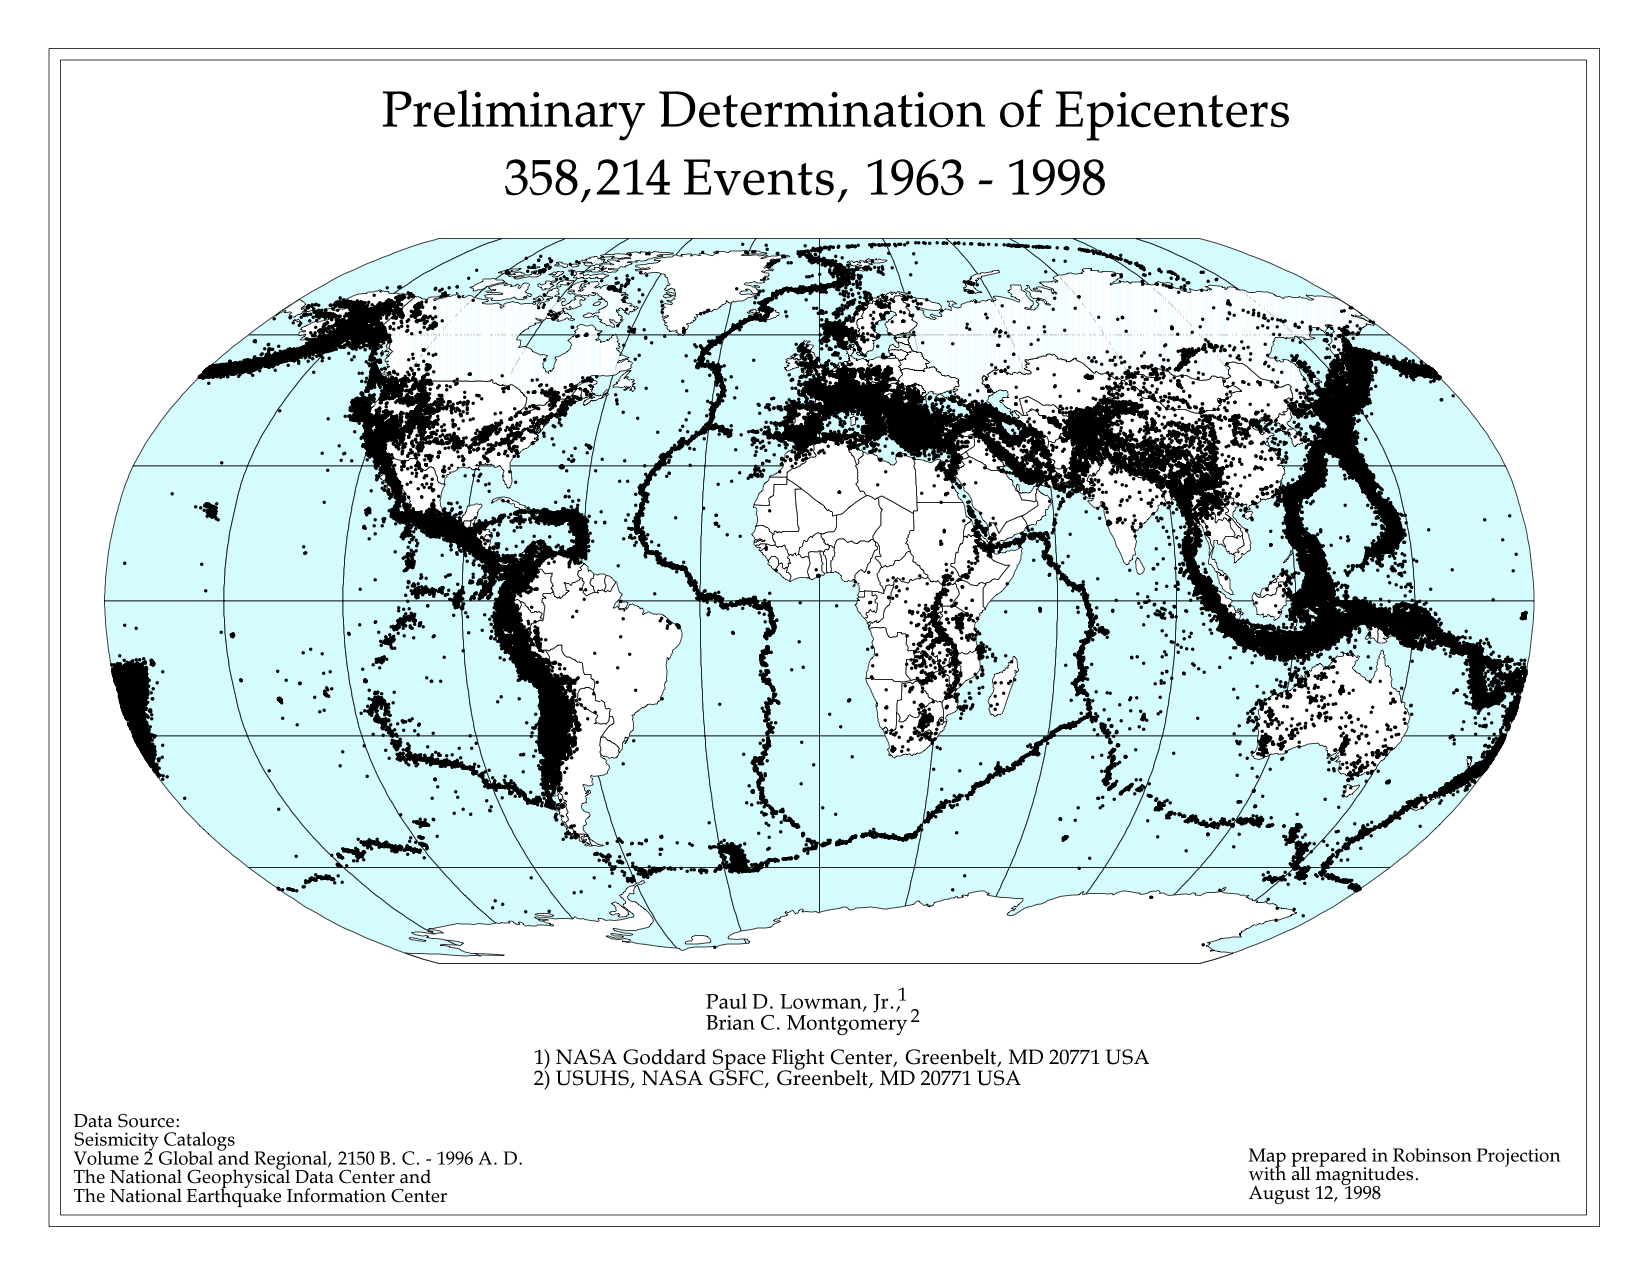
\includegraphics[width=0.80\textwidth]{global_pde_mag_all}
   \caption[Mapa Mundial de Epicentros 1963-1998]
   		   {Mapa Mundial de Epicentros 1963-1998\footnotemark} 
   \label{f:global_epicenters}
\end{figure} 
\footnotetext{\citet{img_world_epicenters}}
 
O padrão apresentado pela \gls{seismic_activity} global foi essencial 
para o desenvolvimento posterior da \gls*{tectonic_plate_theory}.

%% ------------------------------------------------------------------------- %%
\subsection{\Gls{tectonic_plate_theory}}
\index{\Gls{tectonic}!\Gls{tectonic_plate_theory}}
\label{sec:02_placas}

A \gls*{tectonic_plate_theory}, desenvolvida na segunda metade do século XX,
cartografava na superfície do globo as \glspl{litho_plate}.


\begin{figure}[H]
   \centering
   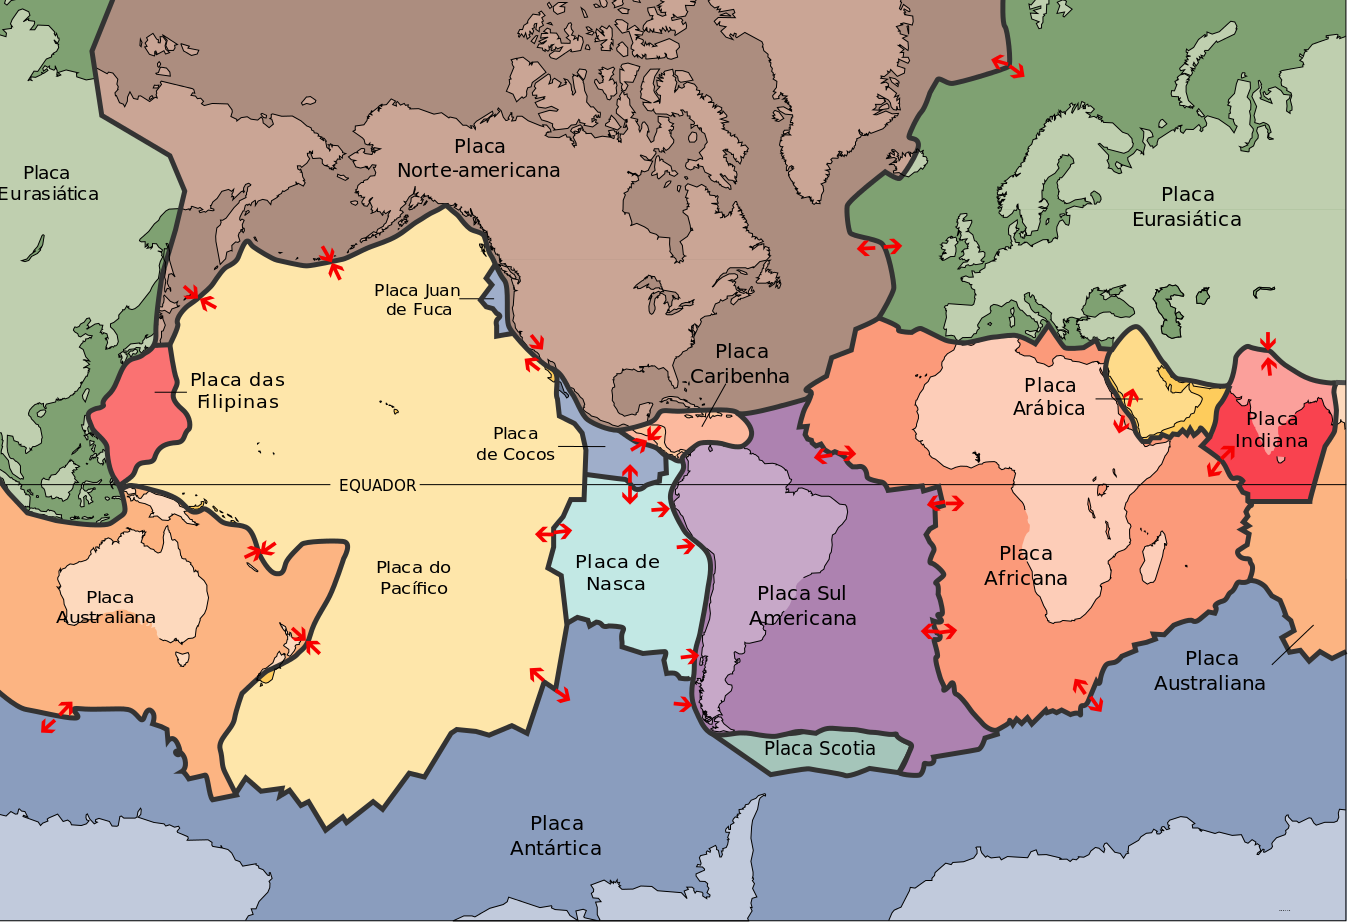
\includegraphics[width=0.80\textwidth]{litho_plates_overview}
   \caption[Cartografia das placas litosféricas]
   		   {Cartografia das placas litosféricas\footnotemark} 
   \label{f:plates_overview}
\end{figure} 
\footnotetext{\citet{img_plates_overview}}
 

As \glspl{litho_plate}, como pode ser visto na figura \ref{f:plates_overview} 
e o conceito de \gls{astenosphere} (\glsdesc{astenosphere}) 
surgem para conformar uma teoria capaz de explicar
uma série de fenômenos tectônicos já observados e ainda não bem explicados na época
de seu desenvolvimento. 


%% ------------------------------------------------------------------------- %%
\subsubsection{Bordas}
\index{\Gls{tectonic_plate_theory}!bordas}
\label{sec:02_bordas}

Nas bordas das \glspl{litho_plate}, a tectônica é mais intensa, 
provocando uma enorme diversidade de fenômenos geológicos de acordo
com o tipo de interação, como ilustrado na figura \ref{f:plate_boundaries}.

\begin{figure}[H]
   \centering
   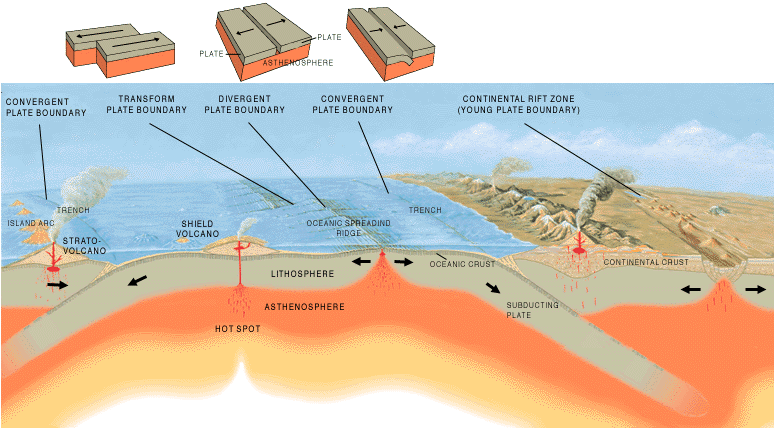
\includegraphics[width=0.80\textwidth]{plate_boundaries}
   \caption[Diferentes tipos de interações entre \glspl{litho_plate} em suas bordas]
   		   {Diferentes tipos de interações entre \glspl{litho_plate} em suas bordas\footnotemark} 
   \label{f:plate_boundaries}
\end{figure} 
\footnotetext{\citet{img_plate_boundaries}}
 
Na figura \ref{f:plate_boundaries} estão ilustrados os diferentes tipos de interação 
entre as \glspl{litho_plate} nas suas bordas, que causam, como já se sabe, a maior
parte dos \glspl{equake} e vulcanismo.

Só na borda das placas é liberada cerca de 95\% da quantidade total da energia 
liberada em \glspl{equake} no globo.

%% ------------------------------------------------------------------------- %%
\subsubsection{Interior}
\index{\Gls{tectonic_plate_theory}!interior}
\label{sec:02_interior}

A dificuldade maior é explicar, com maior detalhe, porque e como são liberados os outros 
5\% do total de energia nos \glspl{equake}, mais raros, no interior das \glspl{litho_plate}.

Não há pleno consenso nem um modelo geral para a explicação do mecanismo de ocorrência dos
sismos no interior das placas, embora sejam conhecidas diversas zonas sísmicas em regiões no interior
de placas, como em Nova Madrid, nos Estados Unidos e também em locais da China e da Austrália para citar alguns.


%% ------------------------------------------------------------------------- %%
\subsection{Sismotectônica}
\index{\gls{tectonic}!\gls{seismotectonic}}
\label{sec:sismotectonica}

A \gls{seismotectonic} é \glsdesc*{seismotectonic}. 

Na prática consiste por um lado, num esforço de compreensão dos
processos geológicos através da observação dos tremores e analogamente, compreender os tremores através da observação
de processos geológicos mensuráveis.  

É fácil notar, portanto, a contribuição dessa disciplina na análise da sismicidade.


\section{Sismicidade}
\index{sismicidade}
\label{sec:sismicidade}

A sismicidade é o estudo da ocorrência de dos tremores. Quando, onde e de que tamanho?!

É sabido que sismos menores são muito mais frequêntes que os grandes tremores de terra
catastróficos.

Tremores de terra, abalos, \glspl{equake}, sismos são a ocorrência de
fenômenos geológicos de ruptura instantânea, de certa dimensão, na
crosta terrestre.


\subsection{Ocorrência}
\index{\gls{equake}!ocorrência}
\label{sec:ocorrencia}
 
Os tremores acontecem num tempo \gls{sym:t}, num lugar \gls{sym:r} e cada um
com seu tamanho \gls{sym:m}.

O local em que se iniciou a ruptura que deu origem ao tremor é um \gls{hypocenter},
enquanto sua projeção na superfície, desconsiderando-se a profundidade, é o \gls{epicenter}.


\subsubsection{Processo de Poisson}
\index{processo de Poisson}
\label{sec:processo_de_Poisson}

Definição do processo\ldots

Críticas\ldots

 
\subsection{Projeção da Ocorrência de Rupturas}
\index{área do trabalho!fundamentos}
\label{sec:fundamentos}

As projeções (\textit{forecasting}) são feitas para se estimar a ocorrência de futuros tremores,
principalmente dos maiores, com grandes chances de provocar perdas.

Nas de curto prazo, estimam-se os próximos tremores
numa escala de dias ou horas considerando uma taxa de sismicidade variável 
com o tempo como no caso dos pré e pós-abalos, ou de quando 
acontece um enxame sísmico, período de maior atividade numa região.
Sua principal aplicação são para tomada de decisões de curto período, 
como evacuação de edifícios.

Nas de longo prazo, foco desse texto, a principal consideração feita é de que a 
\gls{seismic_rate} não varie ao longo do tempo, servindo para estimar as acelerações 
provovadas por tremores que possam ocorrer,
mesmo que muito raramente, de grandes proporções. Suas aplicações fazem sentido quando
se deseja saber o nível de segurança e resistência estrutural que devem ser impostos 
às edificações em geral, ou o valor de um contrato de resseguro de plataformas de petroleo,
ou outros grandes investimentos industriais, como usinas nucleares.

 
\subsection{Magnitude - Tamanho da Ruptura}\index{área do
trabalho!fundamentos}
\label{sec:risco_sismico}

A magnitude de um tremor de terra, é um valor medido numa escala que busca
refletir a energia liberada pelo sismo como sendo proporcional à área
e ao deslocamento da ruptura geológica que o originou.

O desenvolvimento das escalas de magnitude para medir o tamanho dos tremores,
iniciou-se experimentalmente com o sismólogo Charges Richter \citep{richter_1935}.

Existem, entretanto, uma série de diferentes escalas de magnitude,
baseadas em diferentes tipos de medidas. A escolha de qual usar fica a critério
de cada operador de rede sismográfica, que geralmente usam escalas diferentes
para diferentes tamanhos dos tremores, ou até mesmo divulgam mais de um tipo para
um mesmo evento.

As escalas, mesmo sendo calibradas de forma a fornecerem valores similares de acordo com seu
intervalo de relevância, apresentam diferenças consideráveis, quando estimadas para um mesmo evento,
podendo comprometer as análises estatísticas formadas a partir de catálogos com essas diferenças.


\subsubsection{Magnitude Richter}
\index{magnitude!Richter}
\label{sec:magnitude_richter}

As classes de escalas de magnitude mais comuns são as que derivam da definição de Richter \citep{richter_1935}
que se baseia no logarítmo da amplitude do registro das ondas sísmicas. Richter definiu a amplitude máxima de sua
escala pela amplitude máxima observada em um sismômetro Wood-Anderson, com período de 0.8 s, registrando a 100km 
do tremor. Na prática existem algumas incertezas e correções que deveriam ser feitas, principalmente por estar intimamente 
relacionada a um equipamento hoje obsoleto, e pelo fato de que sismos locais (a menos de 100km) têm sua magnitude melhor calculada
usando suas frequencias maiores que as registráveis pelo sismômetro da época.


Outras escalas foram desenvolvidas a partir da medida da amplitude máxima de determinadas fases 
(diferentes tipos de onda sísmica), que apresentam bons resultados para a maior parte dos sismos,
mas não refletem com precisão o tamanho dos maiores, e mais destrutivos eventos, com magnitude acima de 7 ou 8.


\subsubsection{Magnitude de Momento Sísmico }\index{área do
trabalho!fundamentos}
\label{sec:risco_sismico}

Esse evento de natureza sismológica ocorre num
instante \gls{sym:t} liberando uma certa quantidade de energia na forma de \glsdesc{sym:M_0}
\gls{sym:M_0} proporcional à \glsdesc{sym:M_W} \gls{sym:M_W} desse evento.

O \glsdesc{sym:M_0} é apresentado na equação \ref{eq:M_0}:

\begin{equation}
	\gls{eqn:M_0}
	\label{eq:M_0}
\end{equation}
\glsdesc*{eqn:M_0}.

O momento sísmico é estimado geralmente pela inversão duplamente acoplada de um tensor de momento aos registros em 
forma de onda do movimento do chão causado pelo terremoto. Ou, em casos de tremores muito bem registrados, ele pode
ser estimado a partir de algum modelo numérico para a ruptura.

A \glsdesc{sym:M_W} \gls{sym:M_W} \citep{hanks_1999} é baseada no 
logarítmo do \glsdesc{sym:M_0} \gls{sym:M_0}, e não se satura no caso de grandes eventos. 
Sua definição é dada pela equação \ref{eq:M_W} 

\begin{equation}
	\gls{eqn:M_W}
	\label{eq:M_W}
\end{equation}
\glsdesc*{eqn:M_W}.


\subsubsection{Intensidade Macrossísmica}
\index{área do trabalho!fundamentos}
\label{sec:risco_sismico}


A intensidade macrossísmica é uma escala para medir, não a energia proporcional
à ruptura que originou o tremor de terra, mas para retratar a percepção humana do
movimento do chão onde quer este tenha produzido seus efeitos.

Uma das mais difundidas é a escala Modificada de Mercalli \citep{richter_1958} apresentada em sua versão simplificada 
na tabela \ref{tab:mercalli}:

\begin{table}[H]
\begin{center}
\begin{scriptsize}
\noindent\begin{tabular}{c|c|p{12cm}}
\hline
Categoria  	& Sensação & Efeitos \\
\hline
I 			&	Imperceptível 	&	Não sentido. Apenas registado pelos sismógrafos.
\\II 		&	Muito fraco 	&	Sentido por um muito reduzido número de pessoas em 
								repouso, em especial pelas que habitam em andares
								elevados.
\\III 		&	Fraco 			&	Sentido por um pequeno número de pessoas. Bem sentido nos andares elevados.
\\IV 		&	Moderado 		&	Sentido dentro das habitações, podendo despertar do sono um pequeno número de pessoas. 
								Nota-se a vibração de
								portas e janelas e das loiças dentro dos armários.
\\V 		&	Forte 			&	Praticamente sentido por toda a população, fazendo acordar muita gente. 
								Há queda de alguns objectos menos estáveis e param os pêndulos dos relógios. 
								Abrem-se pequenas fendas nos estuques das paredes.
\\VI 		&	Bastante forte 	&	Provoca início de pânico nas populações. Produzem-se leves danos nas habitações, 
								caindo algumas chaminés. O mobiliário menos pesado é deslocado.
\\VII 		&	Muito forte 	&	Caem muitas chaminés. Há estragos limitados em edifícios de boa construção, 
								mas importantes e generalizados nas construções mais frágeis. 
								Facilmente perceptível pelos condutores de veículos automóveis em trânsito. 
								Desencadeia pânico geral nas populações.
\\VIII 		&	Ruinoso  		&	Danos acentuados em construções sólidas. Os edifícios de muito boa construção 
								sofrem alguns danos. Caem campanários e chaminés de fábricas.
\\IX 		&	Desastroso 		&	Desmoronamento de alguns edifícios. Há danos consideráveis em construções muito sólidas.
\\X 		&	Destruidor 		&	Abrem-se fendas no solo. Há cortes nas canalizações, torção nas vias de caminho 
								de ferro e empolamentos e fissuração nas estradas.
\\XI 		&	Catastrófico 	&	Destruição da quase totalidade dos edifícios, mesmo os mais sólidos. 
								Caem pontes, diques e barragens. Destruição das redes de canalização e das vias de comunicação. 
								Formam-se grandes fendas no terreno, acompanhadas de desligamento. Há grandes escorregamentos de terrenos.
\\XII 		&	Cataclismo 		&	Destruição total. Modificação da topografia. Nunca foi presenciado no período histórico. \\
\hline
\end{tabular}
\caption{Escala simplificada de intensidade sísmica, modificada em 1956 a partir da escala original de Giuseppe Mercalli de 1902}
\label{tab:mercalli}
\end{scriptsize}
\end{center}
\end{table}
Existem estudos \citep{bakun_1999} que propõem a inferência sobre o tamanho da ruptura, e sua
magnitude, a partir de observações macrossísmicas, ou dos efeitos relatados pela escala de intenside, georreferenciados.



%% ------------------------------------------------------------------------- %%
\subsection{Catálogos}
\index{catálogos}
\label{sec:catalogos}


%% ------------------------------------------------------------------------- %%
\subsubsection{Epicentros}\index{área do trabalho!fundamentos}
\label{sec:fundamentos}

Epicentros $ E : {(x,y,t,m)}$

Com incertezas

$ E : {(x,\sigma_x,y,\sigma_y,t,\sigma_t,m,\sigma_m)}$


%% ------------------------------------------------------------------------- %%
\subsubsection{Hipocentros}\index{área do trabalho!fundamentos}
\label{sec:fundamentos}

hipocentros $ H : {(x,y,z,t,m)}$

Com incertezas

hipocentros $ H : {(x,\sigma_x,y,\sigma_y,z,\sigma_z,t,\sigma_t,m,\sigma_m)}$


\subsection{Distribuição de Frequência e Magnitudes}\index{área do
trabalho!fundamentos}
\label{sec:risco_sismico}

À uma primeira abordagem estatística, seria conveniente analisar a frequência de
ocorrencia dos sismos.

\subsubsection{Gutemberg-Richter MFD}\index{área do
trabalho!fundamentos}
\label{sec:risco_sismico}

Gutemberg e Richter, por terem desenvolvido à escala de tamanho dos
tremores, foram os primeiros a analisar sua frequência de ocorrencia com estes
mesmos tamanhos.

A observação de que a forma da sua distribuição se caracterizava por uma 
XXXXX, é utilizada até hoje para a estimativa da ocorrencia de tremores futuros.



\subsubsection{Truncated MFD}\index{área do
trabalho!fundamentos}
\label{sec:risco_sismico}

Como variações ou critérios de contorno, algumas distribuições foram surgindo,
como por exemplo a distribuição truncada de magnitude e frequência (TMFD):


FORMULAS


GRAFICO



\subsubsection{Tapered MFD}\index{área do
trabalho!fundamentos}
\label{sec:risco_sismico}


Existe também distribuições que terminam suavemente em magnitudes menos
elevadas, sugerindo a raridade dos fenomenos geológicos ou o tempo escasso de
observação.


\subsubsection{Exponential cutoff MFD}\index{área do
trabalho!fundamentos}
\label{sec:risco_sismico}

Entretanto, fenômenos de maiores magnitudes podem ter sido noticiados em
maior quantidade sugerindo distribuições um pouco mais alongadas:

GRAFICO

FORMULA



\section{Taxa de Sismicidade}\index{área do
trabalho!fundamentos}
\label{sec:risco_sismico}


Texto texto texto texto texto texto texto texto texto texto texto texto texto
texto texto texto texto texto texto texto texto texto texto texto texto texto
texto texto texto texto texto texto texto texto texto texto texto texto texto


\subsubsection{Magnitude de Completude}\index{área do
trabalho!fundamentos}
\label{sec:risco_sismico}

A magnitude de completude\ldots 

texto texto texto texto texto texto texto texto texto texto texto texto texto


GRAFICO

FORMULA



\subsubsection{Valor-b}\index{área do
trabalho!fundamentos}
\label{sec:risco_sismico}


Texto texto texto texto texto texto texto texto texto texto texto texto texto
texto texto texto texto texto texto texto texto texto texto texto texto texto
texto texto texto texto texto texto texto texto texto texto texto texto texto


\subsubsection{Valor-a}\index{área do
trabalho!fundamentos}
\label{sec:risco_sismico}



Texto texto texto texto texto texto texto texto texto texto texto texto texto
texto texto texto texto texto texto texto texto texto texto texto texto texto
texto texto texto texto texto texto texto texto texto texto texto texto texto




\section{Risco Sísmico}\index{área do trabalho!fundamentos}
\label{sec:risco_sismico}

-> risk = ( hazard, 
			exposition, 
			vulnerability)


Texto texto texto texto texto texto texto texto texto texto texto texto texto
texto texto texto texto texto texto texto texto texto texto texto texto texto
texto texto texto texto texto texto texto texto texto texto texto texto texto



\section{Ameaça Sísmica}\index{área do trabalho!fundamentos}
\label{sec:ameaca_sismica}

-> hazard = seismic sources, 
			rupture occurence, 
			ground motion prediction 



Texto texto texto texto texto texto texto texto texto texto texto texto texto
texto texto texto texto texto texto texto texto texto texto texto texto texto
texto texto texto texto texto texto texto texto texto texto texto texto texto



\section{Análise Probabilistica de Ameaça Sísmica}\index{área do
trabalho!fundamentos}
\label{sec:psha}


cornell, mcguire ?!?


Texto texto texto texto texto texto texto texto texto texto texto texto texto
texto texto texto texto texto texto texto texto texto texto texto texto texto
texto texto texto texto texto texto texto texto texto texto texto texto texto



%% ------------------------------------------------------------------------- %%
\subsection{Caracterização de Fontes Sísmicas}
\index{ácido!nucléico}\index{nucleotídeos}
\label{sec:fontes}

cornell, mcguire ?!?


Texto texto texto texto texto texto texto texto texto texto texto texto texto
texto texto texto texto texto texto texto texto texto texto texto texto texto
texto texto texto texto texto texto texto texto texto texto texto texto texto



\subsubsection{Tipologia e Representação Geométrica}
\index{ácido!nucléico}\index{nucleotídeos}
\label{sec:fontes_tipologia}


\subsubsection{Falha Complexa}
\index{ácido!nucléico}\index{nucleotídeos}
\label{sec:fonte_falha_complexa}


Texto texto texto texto texto texto texto texto texto texto texto texto texto
texto texto texto texto texto texto texto texto texto texto texto texto texto
texto texto texto texto texto texto texto texto texto texto texto texto texto



\subsubsection{Falha Simples}
\index{ácido!nucléico}\index{nucleotídeos}
\label{sec:fonte_falha_complexa}



Texto texto texto texto texto texto texto texto texto texto texto texto texto
texto texto texto texto texto texto texto texto texto texto texto texto texto
texto texto texto texto texto texto texto texto texto texto texto texto texto



\subsubsection{Área}
\index{ácido!nucléico}\index{nucleotídeos}
\label{sec:fonte_falha_complexa}


Texto texto texto texto texto texto texto texto texto texto texto texto texto
texto texto texto texto texto texto texto texto texto texto texto texto texto
texto texto texto texto texto texto texto texto texto texto texto texto texto



\subsubsection{Pontos}
\index{ácido!nucléico}\index{nucleotídeos}
\label{sec:fonte_falha_complexa}


Texto texto texto texto texto texto texto texto texto texto texto texto texto
texto texto texto texto texto texto texto texto texto texto texto texto texto
texto texto texto texto texto texto texto texto texto texto texto texto texto



\subsection{Caracterização}
\index{ácido!nucléico}\index{nucleotídeos}
\label{sec:fontes}



Texto texto texto texto texto texto texto texto texto texto texto texto texto
texto texto texto texto texto texto texto texto texto texto texto texto texto
texto texto texto texto texto texto texto texto texto texto texto texto texto



\subsubsection{Ocorrência de Sismicidade}
\index{ácido!nucléico}\index{nucleotídeos}
\label{sec:fontes}


Texto texto texto texto texto texto texto texto texto texto texto texto texto
texto texto texto texto texto texto texto texto texto texto texto texto texto
texto texto texto texto texto texto texto texto texto texto texto texto texto


\subsubsection{Ocorrência de Sismicidade}
\index{ácido!nucléico}\index{nucleotídeos}
\label{sec:fontes}




Texto texto texto texto texto texto texto texto texto texto texto texto texto
texto texto texto texto texto texto texto texto texto texto texto texto texto
texto texto texto texto texto texto texto texto texto texto texto texto texto



\subsubsection{Caracterização de Fontes Sísmicas}
\index{ácido!nucléico}\index{nucleotídeos}
\label{sec:fontes}



Texto texto texto texto texto texto texto texto texto texto texto texto texto
texto texto texto texto texto texto texto texto texto texto texto texto texto
texto texto texto texto texto texto texto texto texto texto texto texto texto





%% ------------------------------------------------------------------------- %%
\subsection{Predição do Movimento do Chão} 
\index{Equação de Predição do Movimento do Chão}
\index{gmpe}
\label{sec:gmpe}


Texto texto texto texto texto texto texto texto texto texto texto texto texto
texto texto texto texto texto texto texto texto texto texto texto texto texto
texto texto texto texto texto texto texto texto texto texto texto texto texto



%% ------------------------------------------------------------------------- %%
\subsection{Cálculo da Curvas de Ameaça} 
\index{curvas ameaça}
\label{sec:curvas_de_ameaca}


Texto texto texto texto texto texto texto texto texto texto texto texto texto
texto texto texto texto texto texto texto texto texto texto texto texto texto
texto texto texto texto texto texto texto texto texto texto texto texto texto

